% Si vous vous demandez à quoi servent les empty \mbox après les paragraphes,
% vous êtes des boulays, apprenez latex.
\subsection{Introduction}
  La théorie des graphes est un domaine entre les mathématiques et
  l'informatique très utilisé dans la résolution de nombreux problèmes.
  
  Nous verrons dans cette section quelques applications des graphes. Une
  dernière application sera vu dans la section~\ref{sec:laby}.

\subsection{Définitions}
  \begin{description}
    \item[Graphe] Un graphe est constitué d'un ensemble de sommets, et d'un
      ensemble d'arêtes (c'est-à-dire des couples de sommets) qui relient ces
      sommets.
      \begin{center}
        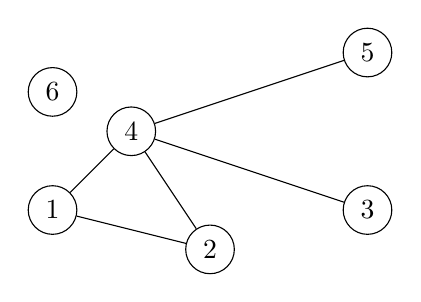
\begin{tikzpicture}[node distance=1.5cm,auto]
          \node[draw, circle] (1) at (0,0) {1};
          \node[draw, circle] (2) at (2,-0.5) {2};
          \node[draw, circle] (3) at (4,0) {3};
          \node[draw, circle] (4) at (1,1) {4};
          \node[draw, circle] (5) at (4,2) {5};
          \node[draw, circle] (6) at (0,1.5) {6};

          \path (2) edge node {} (1);
          \path (4) edge node {} (2);
          \path (4) edge node {} (3);
          \path (1) edge node {} (4);
          \path (4) edge node {} (5);
        \end{tikzpicture}
      \end{center}
    \item[Graphe connexe] Un graphe est dit connexe quand on peut aller de
      n'importe quel sommet vers n'importe quel autre sommet en suivant des
      arrêtes.
      \begin{center}
        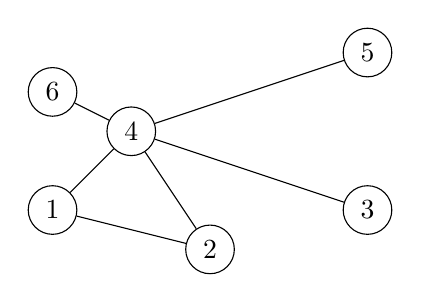
\begin{tikzpicture}[node distance=1.5cm,auto]
          \node[draw, circle] (1) at (0,0) {1};
          \node[draw, circle] (2) at (2,-0.5) {2};
          \node[draw, circle] (3) at (4,0) {3};
          \node[draw, circle] (4) at (1,1) {4};
          \node[draw, circle] (5) at (4,2) {5};
          \node[draw, circle] (6) at (0,1.5) {6};

          \path (2) edge node {} (1);
          \path (4) edge node {} (2);
          \path (4) edge node {} (3);
          \path (1) edge node {} (4);
          \path (4) edge node {} (5);
          \path (4) edge node {} (6);
        \end{tikzpicture}
      \end{center}
    \item[Graphe orienté] Un graphe orienté n'est pas constitué d'arêtes mais
      d'arcs (des paires de sommets).
      \begin{center}
        \begin{tikzpicture}[->, >=stealth', shorten >=1pt, node
          distance=1.5cm,auto]
          \node[draw, circle] (1) at (0,0) {1};
          \node[draw, circle] (2) at (2,-0.5) {2};
          \node[draw, circle] (3) at (4,0) {3};
          \node[draw, circle] (4) at (1,1) {4};
          \node[draw, circle] (5) at (4,2) {5};
          \node[draw, circle] (6) at (0,1.5) {6};

          \draw[arrows={-triangle 90}] (2) --++ (1);
          \draw[arrows={-triangle 90}] (4) --++ (2);
          \draw[arrows={-triangle 90}] (4) --++ (3);
          \draw[arrows={-triangle 90}] (1) --++ (4);
          \draw[arrows={triangle 90-triangle 90}] (4) --++ (5);
        \end{tikzpicture}
      \end{center}
    \item[Graphe complet] Un graphe est dit complet quand tout ses sommets sont
      reliés deux à deux par une arrête. Le nombre de d'arêtes d'un tel graphe
      est alors $\frac {n(n-1)} 2$.
      \begin{center}
        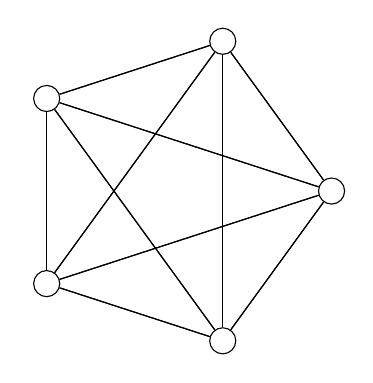
\begin{tikzpicture}[node distance=1.5cm,auto]
          \foreach \x in {0, 72, ..., 359}
            \node[draw, circle] (\x) at (\x:2) {};

          \foreach \x in {0, 72, ..., 359}
            \foreach \y in {0, 72, ..., 359}
              \path (\x) edge node {} (\y);
        \end{tikzpicture}
      \end{center}
    \item[Degré d'un sommet] Le degré d'un sommet est le nombre d'arêtes
      incidentes à ce sommet.
  \end{description}

\subsection{Modélisation mathématique}
Il existe plusieurs moyens de représenter des graphes. Parmi ceux-ci,
le plus simple est la matrice d'adjacence, où l'on stocke une matrice
de taille $n\times n$ ($n$ étant le nombre de sommets), dont chaque
colonne et chaque rangée représente un sommet. La case $i, j$ de la
matrice contient un $1$ si les sommets $i$ et $j$ sont reliés par une
arête (ou un arc dans le bon sens, dans le cas orienté). Évidemment,
cette représentation est loin d'être efficace, la mémoire utilisée
étant exponentielle quand le nombre de sommets du graphe
augmente. Toutefois, elle peut servir pour certains
algorithmes. Notamment, un algorithme de recherche de chemin peut
multiplier la matrice d'adjacence par elle-même $m$ fois : alors, il
existera un chemin de taille $m$ entre deux sommets si la case
correspondante contient un $1$.

  On peut également représenter les graphes par une liste de sommets,
  chacun ayant une liste d'arêtes.
  En mémoire, cette structure est donc constituée d'une liste de pointeurs
  vers des sommets. Les sommets contenant une liste de pointeurs vers des
  arêtes. Chaque arête dispose d'un pointeur vers chaque sommet extrémité.
  Cette structure est évidemment plus efficace, car elle ne stocke que
  les informations nécessaires.


\subsection{Graphes eulériens}
  \subsubsection{Analyse mathématique}
    Un graphe eulérien est un graphe contenant un cycle eulérien, c'est-à-dire
    une chaine parcourant toutes les arêtes du graphe une et une seule fois, en
    revenant au sommet de départ.

    \begin{description}
      \item[Théorème d'Euler] Un graphe connexe est eulérien si et seulement si
        chacun de ses sommets est de degré pair.
    \end{description}

    Un graphe semi-eulérien, quant à lui, contient une chaine eulérienne:
    celle-ci passe également par toutes les arêtes du graphe une seule et
    unique fois, mais ne retourne pas au sommet de départ. Le théorème précédent
    se généralise alors aux graphes semi-eulériens: un graphe connexe est
    semi-eulérien si et seulement tous ses sommets sauf deux sont associés à un
    nombre pair d'arêtes. Dans ce cas, la chaine eulérienne aura pour départ
    l'un des deux sommets associés à un nombre impair d'arêtes et pour sommet
    d'arrivée le deuxième.

  \subsubsection{Méthode de résolution}
    Afin de trouver une chaine ou un cycle eulérien dans un graphe, on peut
    utiliser deux méthodes: une méthode qui teste toutes les possibilités, et
    une autre plus intelligente et moins couteuse.

    \paragraph{Matrices latines}
      La première méthode (voir algorithme~\ref{alg:meth_mat_lat}) est inspirée
      des matrices latines. Chaque coefficient de la matrice sera un ensemble
      de chaines, une chaine étant elle-même une liste de sommets. La matrice
      latine de notre graphe sera la matrice $M$ dont chaque coefficient
      $m_{i,j}$ vaudra:
      \begin{itemize}
        \item l'ensemble vide si le nœud $i$ n'est pas relié au nœud $j$ dans
          le graphe;
        \item un ensemble contenant pour unique élément la chaine  $[N_i,N_j]$
          si les nœuds $i$ et $j$ sont reliés (où $N_k$ représente le nœud
          $k$).
      \end{itemize}

      Nous définissions ensuite un produit sur les coefficients d'une telle
      matrice (voir algorithmes~\ref{alg:prod_mat} et~\ref{alg:prod_chaine}). Le
      produit de deux chaines sera:
      \begin{itemize}
        \item nul si le dernier nœud de la première chaine n'est pas le premier
          nœud du deuxième;
        \item la concaténation des deux chaines sinon.
      \end{itemize}

      Le produit de deux ensembles de chaines sera l'ensemble contenant les
      produits de chaque couple de nœuds.

      Pour tout $k$ entier naturel, le coefficient $(i,j)$ de la matrice $M^k$
      représentera l'ensemble des chaines de longueur $k$ reliant les nœuds $i$
      et $j$.

      Puisque une chaine eulérienne passe une unique fois par chaque arête, il
      suffira de calculer la matrice latine élevée à cette puissance pour
      trouver sur sa diagonale l'ensemble des cycles possibles. En éliminant à
      chaque produit les chaines qui passent plusieurs fois par la même arête,
      on trouve l'ensemble des cycles eulériens.

      La complexité de cet algorithme est exponentielle, calculer la puissance
      de la matrice latine revient en fait à calculer chaque chaine possible dans
      le graphe, et tester si elle est un cycle eulérien ou non.

    \paragraph{Algorithme d'Euler}
      La deuxième méthode, basée sur l'algorithme d'Euler est nettement plus
      efficace. Une fonction récursive cherche un cycle eulérien d'un
      sous-graphe de notre graphe de départ, puis s'appelle récursivement sur
      chacun des sommets parcourus par cette chaine, dans le graphe où l'on a
      supprimé les arêtes déjà parcourues. En reconstruisant ces cycles
      astucieusement, on parvient à trouver un cycle eulérien de complexité
      linéaire en le nombre d'arêtes du graphe.

    \begin{algorithm}
      \KwIn{un graphe}
      \KwOut{%
        la liste des cycles ou chaines eulériens si le graphe est eulérien
        semi-eulérien ou la liste vide sinon
      }
      \Begin{%
        \tcc{Construction de la matrice latine du graphe}
        construire une matrice à n lignes et n colonnes\;
        remplir la matrice de listes vides\;
        \For{chaque nœud du graphe}{%
          \For{chaque arête sortant de ce nœud}{%
            ajouter la liste [noeud de départ, noeud d'arrivée] à la case de
            la matrice correspondante\;
          }
        }
        n $\leftarrow$ le nombre d'arêtes total du graphe\;
        calculer la puissance $(n-1)$ième de la matrice

        \For{chaque coefficient de la matrice ainsi calculée}{%
          \If{le coefficient n'est pas nul}{%
            concaténer ce coefficient à la variable de retour\;
          }
        }
      }
      \caption{Méthode de la matrice latine}
      \label{alg:meth_mat_lat}
    \end{algorithm}

    \begin{algorithm}
      \KwIn{$A$ et $B$ deux matrices latines}
      \KwOut{le produit de ces deux matrices}
      \Begin{%
        construire la matrice de retour à n lignes et n colonnes\;
        initialiser chaque coefficient de cette matrice à la liste vide\;

        \For{chaque coefficient de la matrice de retour}{%
          \For{$k$ allant de $1$ jusqu'à $n$}{%
            calculer les chaines produits entre a(i,k) et b(k,j)\;
            ajouter au coefficient de la matrice ces chaines\;
          }
        }
      }
      \caption{Produit matriciel}
      \label{alg:prod_mat}
    \end{algorithm}

    \begin{algorithm}
      \KwIn{liste\_1 et liste\_2 deux listes de chaine}
      \KwOut{une liste de chaines}
      \Begin{%
        créer une liste de chaine vide (liste de retour)\;
        \For{$i$ dans liste\_1}{%
          \For{$j$ dans liste\_2}{%
            construire la chaine résultante de la concaténation de $i$ et $j$
            (en enlevant le nœud présent deux fois)\;
            construire un ensemble de chaine vide\;
            \For{$k$ allant de $1$ à la longueur de la chaine construit}{%
              construire la chaine élémentaire menant du nœud $k$ au nœud $k+1$\;
              \If{cette chaine n'est pas dans l'ensemble}{%
                ajouter cette chaine dans l'ensemble\;
              }
              \Else{%
                rendre la chaine nulle\;
                sortir de la boucle\;
              }
            }
          }
          \Si{le chaine n'est pas nulle}{%
            concaténer la chaine trouvée à la liste de retour
          }
        }
      }
      \caption{Produit entre listes de chaines (coefficients de matrices
      latines)}
      \label{alg:prod_chaine}
    \end{algorithm}

\subsection{Graphes hamiltoniens}
  \subsubsection{Analyse mathématique}
    Un graphe hamiltonien (resp.\ semi-hamiltonien) est un graphe sur lequel on
    peut trouver un cycle (resp.\ une chaine) passant par tout les sommets une
    et une seule fois. Ce problème est donc celui d'un enfant qui souhaiterait
    visiter de manière unique toutes les salles d'un musée.

    Le problème de savoir si un graphe est (semi-)hamiltonien est NP-complet,
    de même que de trouver un cycle ou une chaine s'il y en a.

    Il existe cependant des conditions suffisantes pour lesquelles on peut
    affirmer qu'un graphe est hamiltonien.

    \begin{description}
      \item[Théorème] Un graphe complet est hamiltonien. C'est une conséquence
        du théorème de Dirac.
      \item[Théorème de Dirac] Un graphe simple à $n$ sommets ($n \ge 3$) dont
        chaque sommet est au moins de degré $\frac{n}{2}$ est hamiltonien.
      \item[Théorème de Ore] Un graphe simple à $n$ sommets ($n \ge 3$) tel que
        la somme des degrés de toute paire de sommets non adjacents vaut au
        moins $n$ est hamiltonien.
      \item[Théorème de Pósa] Un graphe simple à $n$ sommets ($n \ge 3$) est
        hamiltonien si:
        \begin{itemize}
          \item pour tout entier $k$ tel que $1 \le k < \frac{n-1}{2}$ le
            nombre de sommets de degré inférieur ou égal à $k$ est inférieur à
            $k$;
          \item le nombre de sommets de degré inférieur ou égal à
            $\frac{n-1}{2}$ est inférieur ou égal à $\frac{n-1}{2}$.
        \end{itemize}
      \item[Fermeture d'un graphe] La fermeture d'un graphe est le graphe
        construit à partir de celui en rajoutant des arrêtes entre chaque
        sommets $a$ et $b$ tel que $\deg(a)+\deg(b) > n$ tant qu'il en existe.
      \item[Théorème de Bondy et Chvátal] Un graphe est hamiltonien si et
        seulement si sa fermeture est hamiltonienne.

        Ce théorème n'est utile que si l'on peut utiliser l'un des théorèmes
        précédents sur la fermeture.
    \end{description}

  \subsubsection{Méthode de résolution}
    Pour tester si un graphe est hamiltonien on peut utiliser les théorèmes
    précédents. Si le graphe ne respecte les conditions d'aucun de ces
    théorèmes, on recherche une chaine hamiltonienne dans ce graphe.

    Pour rechercher une chaine hamiltonienne dans un graphe, on pourrait
    chercher parmi toutes les chaines possibles. La complexité d'un tel
    algorithme (voir algoritme~\ref{alg:hamil}) dans le pire des cas est donc
    très mauvaise: $O(n!)$. Comme on peut s'arrêter dès qu'on a trouvé une
    chaine sans devoir tester toutes les autres chaines possibles, la
    complexité moyenne sera inférieure.

    \begin{algorithm}
      \KwIn{un graphe}
      \KwIn{un sommet de départ optionnel node\_from}
      \KwIn{un ensemble (éventuellement vide) de nœuds déjà parcouru
      nodes\_done}
      \KwOut{une chaine hamiltonienne sous la forme d'une liste ordonnée de
      sommets, ou None s'il n'en existe pas}

      \Begin{%
        \If{node\_from n'a pas été fourni}{%
          node\_from $\leftarrow$ un nœud du graphe\;
        }
        ajouter node\_from à nodes\_dones\;

        \If{cardinal(node\_from) == ordre(graphe)}{%
          \Return{[node\_from]}
        }

        \For{chaque arête dans le graphe}{%
          autre $\leftarrow$ le sommet opposé à node\_from par rapport à cette
          arête\;
          \If{autre dans nodes\_done}{%
            passer à la prochaine arête
          }
          appeler la fonction récursivement avec le graphe, node\_from et
          nodes\_dones comme paramètres\;
          \If{la liste retournée est non-vide}{%
              y ajouter node\_from au début et la retourner\;
          }
        }
      }
      \caption{Recherche de chaine hamiltonienne}
      \label{alg:hamil}
    \end{algorithm}

\subsection{Problème du postier chinois}
  \subsubsection{Analyse mathématique}
    Le problème du postier chinois consiste à trouver la chaine la plus courte
    dans un graphe connexe non-orienté passant au moins une fois par chaque
    arête, et revenant à son point de départ.

    Ce problème est donc celui du facteur qui souhaite réaliser une tournée
    la plus rapidement possible en passant par toutes les rues et retournant
    à la poste.

    Ce problème peut être réduit à la recherche d'un couplage parfait de cout
    minimum, que peut être résolu en temps polynomial dans le cas général.

    \begin{description}
      \item[Couplage] Un couplage d'un graphe est un ensemble d'arêtes de ce
        graphe qui n'ont pas de sommets en commun.
      \item[Couplage Parfait] Un couplage parfait est un couplage tel que tout
        sommet du graphe est présent une fois et une seule dans le couplage.
      \item[Clique] Une clique est un ensemble de sommets deux à deux
        adjacents.
    \end{description}

  \subsubsection{Méthode de résolution}
    On remarque que dans le cas d'un graphe eulérien, il suffit d'appliquer
    l'algorithme d'Euler (voir algorithmes~\ref{alg:euler}
    et~\ref{alg:couplage} pour avoir la chaine voulue.

    Dans les autres cas, la méthode de résolution consiste à transformer le
    graphe en graphe eulérien, en ajoutant des arêtes. Une méthode possible
    est la suivante:
    \begin{enumerate}
      \item on crée d'abord le graphe partiel contenant uniquement les sommets
        de degré impair;
      \item on transforme ensuite ce graphe en clique: pour chaque couple de
        sommets non reliés entre eux, on crée une arête les rejoignant,
        de poids égal au cout le plus faible possible pour rejoindre ces
        sommets dans le graphe initial (ceci se calcule facilement avec
        l'algorithme de Dijkstra);
      \item on cherche le couplage parfait de cout minimum en utilisant des
        algorithmes comme celui d'Edmonds. On peut aussi tester simplement
        toutes les possibilités;
      \item pour chaque arête de cet ensemble, on double la chaine la plus
        courte reliant les sommets reliés par cette arête dans le graphe initial;
      \item on obtient alors un graphe eulérien, sur lequel on applique
        l'algorithme d'Euler.
    \end{enumerate}

    \begin{algorithm}
      \KwIn{Un graphe non-orienté et connexe g}
      \KwOut{le cycle le plus court permettant de visiter toutes les arêtes de
      g}

      \Begin{%
        \tcc{Création du graphe partiel}
        \For{chaque sommet de g}{%
          \If{le sommet est de degré impair}{%
            créer le sommet dans graphe\_partiel\;
          }
        }
        \For{chaque arête de g}{%
          \If{ses 2 sommets sont dans graphe\_partiel}{%
            créer la même arête dans graphe\_partiel\;
          }
        }

        \tcc{Transformation en clique}
        \For{chaque couple de sommet (s1, s2) dans graphe\_partiel}{%
          \If{il n'y a pas d'arête reliant s1 et s2}{%
            $(cout, chaine) = dijkstra(s1, s2)$\;
            créer l'arête reliant s1 et s2 dans graphe\_partiel, de cout cout\;
          }
        }

        $couplage, cout = aux(ensemble vide, ensemble vide, 0)$\;

        \For{chaque arête dans couplage}{%
          $(s1, s2) =$ sommets reliés par arête dans g\;
          $(cout, chaine) = dijkstra(s1, s2)$\;
          \For{chaque arête dans chaine}{%
            doubler cette arête dans g\;
          }
        }

        \Return{le cycle eulérien de g}
      }
      \label{alg:euler}
      \caption{TODO: trouver un titre}
    \end{algorithm}

    \begin{algorithm}
      \KwIn{arêtes, sommets\_visités, cout}
      \Begin{%
        \If{sommets\_visites contient tous les sommets de graphe\_partiel}{%
          \Return{(arêtes, cout)}
        }
        \Else{%
          $meilleur\_couplage = Vide$\;
          $meilleur\_cout = 0$\;
          \For{chaque arête de graphe\_partiel}{%
            \If{les 2 sommets de l'arête ne sont pas dans sommets\_visites}{%
              arêtes\_copie = copie de arêtes\;
              sommets\_visites\_copie = copie de sommets\_visites\;

              ajouter arête dans arêtes\_copie\;
              couplage, cout = aux(arêtes\_copie, sommets\_visites\_copie, cout +
              cout de arête)\;

              \If{meilleur\_couplage = Vide ou meilleur\_cout > cout}{%
                meilleur\_couplage = couplage\;
                meilleur\_cout = cout\;
              }
            }
          }
          \Return{(meilleur\_couplage, meilleur\_cout)}
        }
      }
      \label{alg:couplage}
      \caption{Recherche du couplage parfait de cout minimum par bruteforce}
    \end{algorithm}

\subsection{Problème du voyageur de commerce}\label{sec:tsp}
  \subsubsection{Analyse mathématique}
    Le problème du voyageur de commerce consiste à chercher un chemin passant
    par tous les sommets du graphe, de longueur minimale.
    Ce problème peut s'illustrer par l'exemple d'une
    fraiseuse qui doit percer des trous dans une plaque le plus
    rapidement possible, ou encore par un car de touristes qui souhaiterait
    trouver l'itinéraire le plus rapide pour visiter un certain nombre de lieux.

    On peut modéliser ce problème par un graphe complet, dont les arêtes ont un
    cout qui correspond à la distance entre chaque sommet, on cherche alors le
    cycle hamiltonien de cout minimal. On sait qu'un tel cycle existe car le
    graphe est complet.

    Cependant trouver un tel cycle est un problème NP-complet~: il n'existe
    donc pas d'algorithme efficace pour trouver ce cycle, à part une recherche
    exhaustive.
    En effet, la seule méthode exacte consisterait à tester toutes les chaines
    hamiltoniennes, et à prendre celle la plus courte, mais le nombre de chaines
    hamiltonniennes croît exponentiellement en fonction du nombre de sommets
    dans le graphe.

    Nous allons donc nous concentrer sur les méthodes approchées de résolution,
    qui peuvent donner de très bons résultats tout en étant rapides.
    Toutefois, le résultat n'est donc pas forcément le plus court.

  \subsubsection{Heuristiques}
    Les heuristiques vont nous permettre de construire un chemin court (par
    rapport au plus court possible), de manière rapide, avec le moins de calcul
    possible.  Étant donné qu'on est confronté à énormément de possibilités
    pendant la recherche, elles vont permettre d'orienter cette dernière, en
    faisant des choix les plus judicieux possibles sur les possibilités à
    explorer.

    \paragraph{Exemple} Une heuristique simple consiste à partir d'un sommet au
    hasard du graphe et d'aller au sommet le plus proche sur lequel on n'est
    pas encore passé (puis à retourner au sommet de départ pour boucler le
    cycle). Cet algorithme est en $O(n)$ et donc rapide. Mais il n'offre
    cependant aucune garantie de résultat, il existe même des graphes pour
    lesquels il donne le pire cycle.

    Plus généralement, chercher parmi les $p$ sommets les plus proches s'avère
    être une solution relativement efficace, avec une complexité en $O(p^n)$
    (donc toujours exponentielle si $p \neq 1$).

    Une méthode purement basée sur cette heuristique consisterait donc à parcourir
    tout le graphe, en allant sur le voisin le plus proche du sommet courant~:

    \begin{algorithm}
      \KwIn{un graphe complet g}
      \KwOut{(cout, cycle) où cycle est un cycle hamiltonien construit selon la
      méthode du plus proche voisin et cout son cout associé sous forme de
      liste de sommets}
      \Begin{%
        cout = 0\;
        cycle = une liste composée d'un sommet de g au hasard\;

        \While{il reste des sommets}{%
          \tcc{On ajoute au cycle le sommet suivant}
          plus\_proche = sommet de g sur lequel on est pas encore passé le
          plus proche du dernier sommet du cycle\;

          cout += cout de plus\_proche au dernier sommet du cycle construit\;
          ajouter plus\_proche au cycle\;
        }

        \tcc{On ferme le cycle}
        cout += cout du dernier au premier sommet de cycle\;
        ajouter le premier sommet de la chaine à cycle\;

        \Return{(cout, cycle)}
      }
      \label{alg:voisin}
      \caption{Plus proche voisin}
    \end{algorithm}

  \subsubsection{Recherche locale}
    Les heuristiques nous donnant des solutions acceptables, choisies avec un
    minimum de «~bon sens~», il est ensuite possible de tenter d'améliorer
    ces solutions, via de la recherche locale.
    Partant d'une solution fournie, on va explorer les solutions voisines
    à cette dernière, afin de voire si on pourrait pas trouver des solutions
    encore meilleures parmi leur voisinage.

    \paragraph{Exemple} Un algorithme de recherche locale adapté au problème
    du voyageur de commerce est le 2-opt (voir algorithme~\ref{alg:2opt}).
    Le principe du 2-opt consiste à tenter d'éliminer les «~boucles~» qui
    pourraient survenir dans le chemin, afin de le rendre plus court.
    \cite{two_opt}

    Ainsi, partant du chemin suivant (qu'on obtiendrait logiquement en suivant
    l'heuristique consistant à aller sur le sommet le plus près):

    \begin{center}
    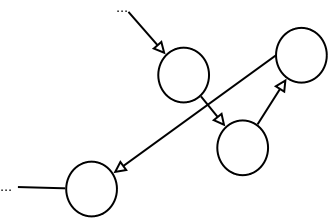
\includegraphics[width=0.3\textwidth]{graphes/2opt1.png}
    \end{center}

    On obtiendrait ceci, en éliminant le croisement:

    \begin{center}
    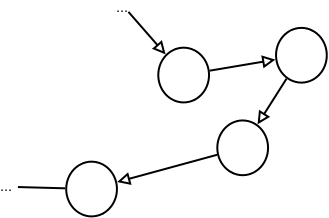
\includegraphics[width=0.3\textwidth]{graphes/2opt2.png}
    \end{center}

    \begin{algorithm}
      \KwIn{un cycle hamiltonien (liste de sommets) et son cout}
      \KwOut{un cycle hamiltonien et son cout inférieur ou égal au coup
      d'entrée}

      \Begin{%
        \For{chaque couple de sommets (a, b) dans le cycle}{%
           $\begin{aligned}
             \text{nouveau\_cout} & \leftarrow
            \text{cout}\\
            &- \text{cout de a à son successeur dans le cycle}\\
            &- \text{cout de b à son successeur dans le cycle}\\
            &+ \text{cout de a à b}\\
            &+ \text{cout du successeur de a au successeur de b dans le
            cycle}\\
          \end{aligned}$\;

          \If{nouveau\_cout < cout}{%
            cout = nouveau\_cout
            cycle = cycle crée en échangeant a et b dans cycle\;
          }
        }
        \Return{(cout, cycle)}
      }
      \caption{2-opt}
      \label{alg:2opt}
    \end{algorithm}

    Il a donc une complexité quadratique du nombre de sommets du cycles.

    L'application du 2-opt sur le chemin obtenu via une heuristique simple peut
    donner des résultats plus proches de la solution optimale qu'on pourrait le
    penser, et la combinaison des deux est donc une bonne méthode.

  \subsubsection{Métaheuristiques}

  Plutôt que d'utiliser une simple heuristique pour trouver une solution à priori plutôt
  bonne, puis d'y appliquer une recherche locale pour tenter de l'améliorer encore,
  il est possible d'utiliser des «~métaheuristiques~».
  Ces algorithmes vont avoir besoin d'heuristiques et de recherche locale, mais vont
  s'en servir en boucle, pour tenter sans cesse de trouver une solution meilleure.

  Ils vont partir explorer différentes parties de l'espace, souvent en guidant
  leur exploration grâce à l'heuristique, et en essayant de retomber sur des
  parties de l'espace les plus intéressantes possibles grâce aux algorithmes de
  recherche locale.

  Il existe énormément de métaheuristiques. En voici quelques uns:
  \begin{description}
  \item[Recherche locale itérée] métaheuristique très simple consistant à
    utiliser une heuristique puis appliquer de la recherche locale pour
    améliorer son résultat.  Ensuite, on perturbe légèrement ce résultat, on
    applique à nouveau une recherche locale et on recommence.
  \item[Recherche tabou] amélioration de la recherche locale itérée, qui va
    utiliser une «~liste taboue~» bannissant toute recherche autour des zones de
    l'espace déjà explorées.
  \item[Recuit simulé] explore d'abord l'espace sans se restreindre aux parties
    donnant des solutions efficaces, puis se restreint de plus en plus au
    voisinage de celles-ci. Converge donc vers les solutions les plus efficaces
    trouvées, puis relâche les contraintes et explore autour de ces dernières,
    quitte à trouver des solutions vraiment moins efficaces. Recommence à se
    contraindre aux plus efficaces, etc\dots
  \item[Algorithmes génétiques] imitent la sélection naturelle, avec une
    population de solutions qui évoluent en mutant et en s'échangeant leurs
    caractéristiques entre elles. On peut même faire évoluer des populations
    séparément avec les modèles en îles, pour avoir plusieurs populations très
    différentes.
  \item[Colonies de fourmis] imitent là encore la nature en simulant des
    phéromones déposées par des fourmis virtuelles, qui orientent la recherche
    au fil du temps.
  \end{description}

  \subsubsection{Conclusion}
    Il est intéressant de constater que les heuristiques, les méthodes de
    recherche locales et les métaheuristiques sont des choses extrêmement
    générales, utilisées pour résoudre énormément de problèmes demandant
    d'explorer un espace extrêmement grand.

    Elles ne sont donc pas propres au voyageur du commerce, même si on a vu
    comment, dans ce cas précis, on pouvait obtenir des résultats corrects en
    se passant de métaheuristiques. On pourrait donc améliorer ces résultats en
    en utilisant.
